\documentclass[ignorenonframetext,10pt,aspectratio=169]{beamer}

\usepackage{umut}
\usepackage{umuttr}
\usepackage{usynsem}
\usepackage[utf8]{inputenc}
\usepackage{uling}
\usepackage{natbib,unatbib}
\usepackage{linguex}
         \renewcommand{\refdash}{}
\usepackage{ubeamer}
\usepackage{verbatim}
\usepackage{adjustbox}

\usepackage{fancyvrb}
\usepackage{tikz-qtree}
\usetikzlibrary{er,positioning}

\title{Finiteness and Case}
\author{\  \\  {\it Partly based on Koeneman \& Zeiljstra (2017)} \\ \vspace{20pt} Umut \"Ozge\\  }

\date{COGS 532: Theoretical Linguistics\\ METU, Informatics}

\begin{document}

\begin{frame}\frametitle{}
\thispagestyle{empty}
\maketitle
\end{frame}

\begin{frame}[t,plain]{Case assignment: Nominative}
\begin{itemize}
		\item Do verbs also assign the nominative case?
\end{itemize}

\ex. She loves her. 

		\vspace{40pt}

\pause

\ex. \a. She caused him to quit his job.
\b. I saw her dancing.

\end{frame}

\begin{frame}[t,plain,fragile]{Finiteness}

		\begin{itemize}
				\item Verbal items that carry tense and/or agreement features are \alert{finite}.
				\item Nominative case assignment is closely associated with finiteness.
		\end{itemize}

\begin{center}
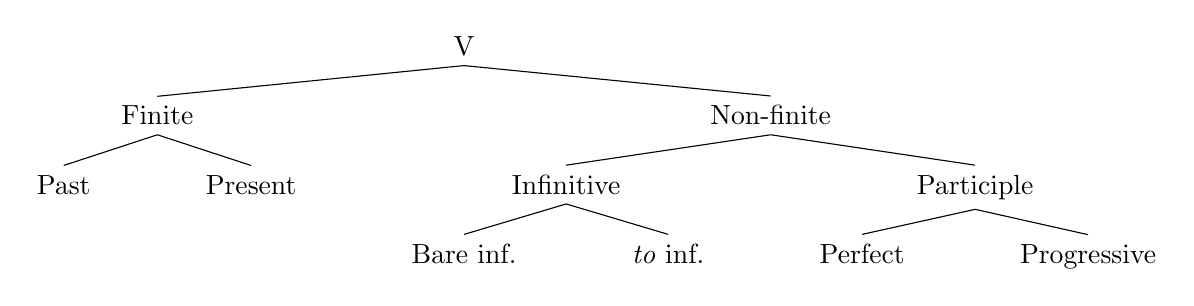
\begin{tikzpicture}
\tikzset{level distance=25pt, sibling distance=35pt}
				\Tree [.V
				[.{Finite}
					[.{Past} ]
					[.{Present} ] ]
				[.{Non-finite} 
					[.{Infinitive}
						[.{Bare inf.} ]
						[.{{\it to }inf.} ]
					]
					[.{Participle} 
						[.{Perfect} ]	
						[.{Progressive} ]	
					]
				] ]
\end{tikzpicture}
\end{center}


\end{frame}

\begin{frame}[t,plain]{Auxiliaries}
				\ex.
				\a. He may leave soon.
				\b. She can face the consequences.
				\b. She must accept the consequences.

				\begin{itemize}

								\item Modal auxiliaries are finite.

				\end{itemize}

\end{frame}

\begin{frame}[t,plain]{Finiteness specification}

\begin{center}
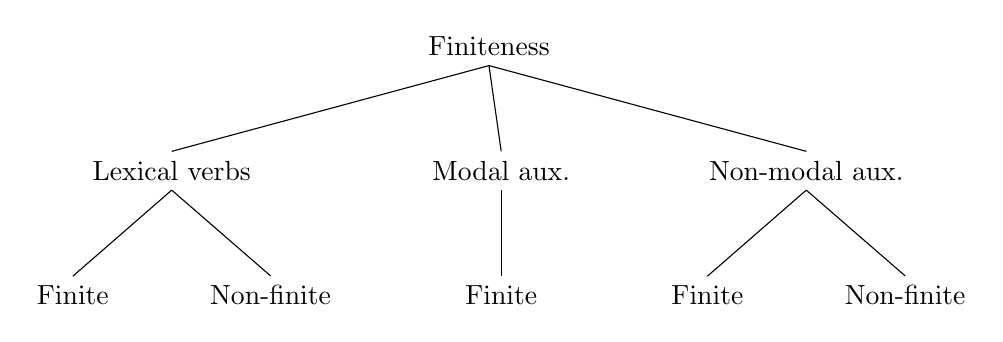
\begin{tikzpicture}
\tikzset{level distance=45pt, sibling distance=30pt}
				\Tree
				[.{Finiteness}
					[.{Lexical verbs}
						[.{Finite} ]
						[.{Non-finite} ] ]
					[.{Modal aux.} {Finite} ]
					[.{Non-modal aux.} 
						[.{Finite} ]
						[.{Non-finite} ] ]
				]
\end{tikzpicture}
\end{center}

\end{frame}

\begin{frame}[t,plain]{Which head assigns the Nominative?}

\adjustbox{valign=t}{
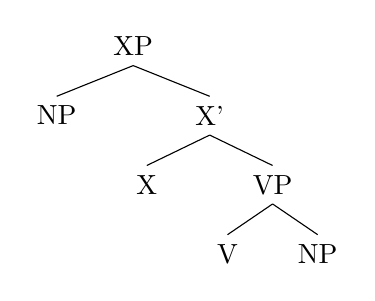
\begin{tikzpicture}
				\tikzset{level distance=25pt, sibling distance=15pt, every tree node/.style={anchor=north}}
				\Tree
				[.{XP}
					[.{NP} ]
					[.{X'} 
						[.{X} ]
						[.{VP}
							[.{V} ] 
							[.{NP} ] 
						]
					]
				]
\end{tikzpicture}}
\hspace{50pt}
\adjustbox{valign=t}{
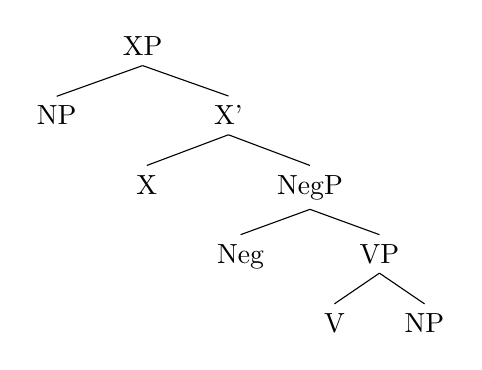
\begin{tikzpicture}
\tikzset{level distance=25pt, sibling distance=15pt}
				\Tree
				[.{XP}
					[.{NP} ]
					[.{X'} 
						[.{X} ]
						[.{NegP} 
							[.{Neg} ]
							[.{VP}
								[.{V} ] 
								[.{NP} ] 
							]
						]
					]
				]
\end{tikzpicture}}
\end{frame}

\begin{frame}[t,plain]{FinP}

				\begin{center}
\begin{tikzpicture}
\tikzset{level distance=35pt, sibling distance=25pt}
				\Tree
				[.{FinP}
					[.{NP} ]
					[.{Fin'} 
						[.{Fin} ]
						[.{NegP} 
							[.{Neg} ]
							[.{VP}
								[.{V} ] 
								[.{NP} ] 
							]
						]
					]
				]
\end{tikzpicture}
				\end{center}

\end{frame}

\begin{frame}[t,plain]{FinP and lexical verbs}
\ex. John loves Mary.

				\begin{center}
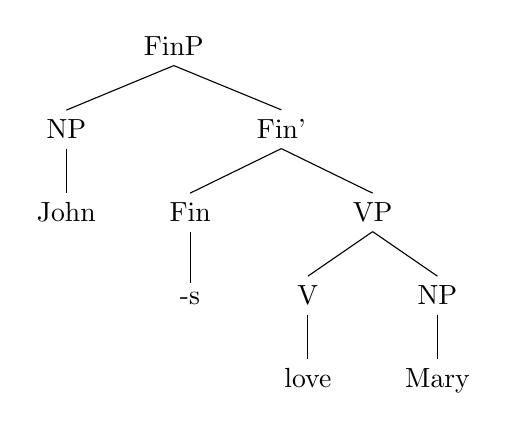
\begin{tikzpicture}
\tikzset{level distance=30pt, sibling distance=20pt}
				\Tree
				[.{FinP}
					[.{NP} John ]
					[.{Fin'} 
						[.{Fin} -s ]
							[.{VP}
								[.{V} love ] 
								[.{NP} Mary ] 
							]
					]
				]
\end{tikzpicture}
				\end{center}

\end{frame}

\begin{frame}[t,plain]{FinP and lexical verbs}

\begin{center}
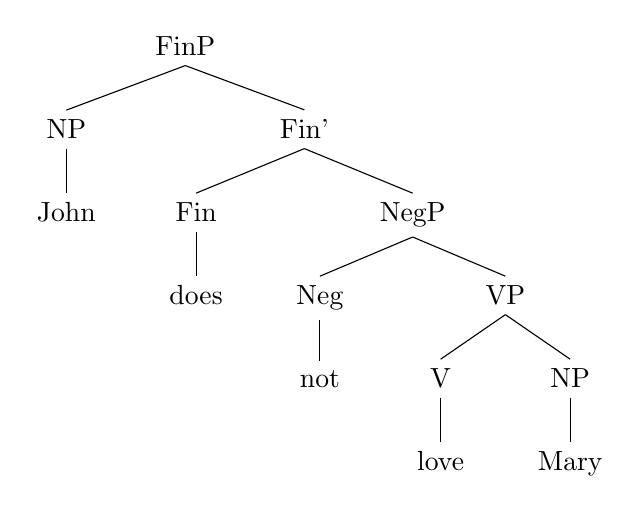
\begin{tikzpicture}
\tikzset{level distance=30pt, sibling distance=20pt}
				\Tree
				[.{FinP}
					[.{NP} John ]
					[.{Fin'} 
						[.{Fin} does ]
						[.{NegP} 
							[.{Neg} not ]
							[.{VP}
								[.{V} love ] 
								[.{NP} Mary ] 
							]
						]
					]
				]
\end{tikzpicture}
\end{center}
\end{frame}

\begin{frame}[t,plain]{{\it to }as non-finite Fin}

				\begin{center}
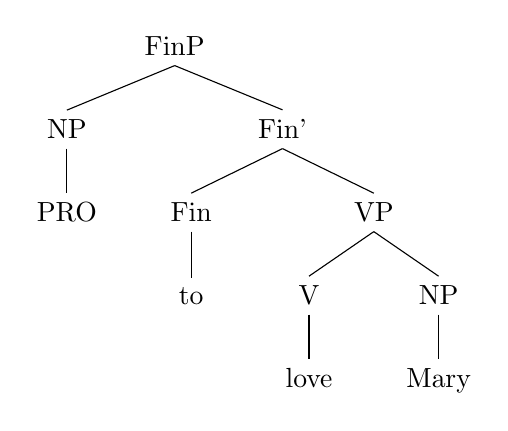
\begin{tikzpicture}
\tikzset{level distance=30pt, sibling distance=20pt}
				\Tree
				[.{FinP}
					[.{NP} PRO ]
					[.{Fin'} 
						[.{Fin} to ]
							[.{VP}
								[.{V} love ] 
								[.{NP} Mary ] 
							]
					]
				]
\end{tikzpicture}
				\end{center}
\end{frame}

\begin{frame}[t,plain]{Finiteness specification}

\begin{center}
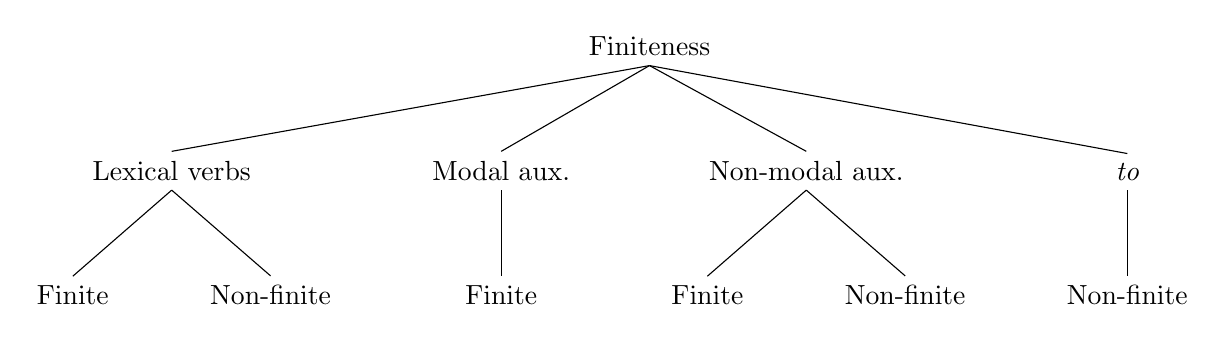
\begin{tikzpicture}
\tikzset{level distance=45pt, sibling distance=30pt}
				\Tree
				[.{Finiteness}
					[.{Lexical verbs}
						[.{Finite} ]
						[.{Non-finite} ] ]
					[.{Modal aux.} {Finite} ]
					[.{Non-modal aux.} 
						[.{Finite} ]
						[.{Non-finite} ] ]
					[.{\it to} Non-finite ]
				]
\end{tikzpicture}
\end{center}

\end{frame}
\begin{frame}[t,plain]{The Case Filter}

		\vspace{40pt}
		Every nominal argument must be assigned either nominative or accusative case.


\end{frame}

\begin{frame}[t,plain]{}

\end{frame}
\end{document}
